\section{Reaktive Programmierung}
\label{section:reaktive_programmierung}
Reaktive Programmierung ist ein ereignisgesteuertes (event-driven) Programmierparadigma.
Der Programmablauf besteht aus Sequenzen von asynchronen Ereignissen (Events).
Die Daten werden als von außen unveränderliche (immutable) Datenströme (Streams) dargestellt.
Sobald es innerhalb des Datenstroms zu Änderungen kommt werden diese als Events durch einen Publisher veröffentlicht.
Diese Events werden dann von einem oder mehreren \verb|Subscribern| konsumiert, welche wiederum weitere Events durch einen
Publisher veröffentlichen können.

Die treibende Kraft bzw. die Stimuli von reaktiven Anwendungen sind also interne Änderungen der Datenströme, wie beispielsweise das
Hinzufügen von Elementen.
Diese Änderungen starten dann den weiteren Programmablauf durch das Auslösen eines oder mehrerer Events.

Die Grundidee orientiert sich am Observer-Pattern und dessen Ausprägung, dem Publish-Subscribe Pattern, erweitert dieses aber
noch um die Benachrichtigungen des Subscribers:
\begin{enumerate}
  \item Sobald keine Events mehr kommen
  \item Wenn ein Fehler aufgetreten ist
\end{enumerate}
Indem Änderungen eines Datenstroms direkt propagiert werden und der Subscriber diesen nicht modifizieren kann, sondern lediglich über Änderungen informiert wird,
können Programme ohne jeglichen Zustand realisiert werden\parencite{Escoffier2017}.

Während ein Datenstrom selber von außen unveränderlich ist, kann aber dennoch der Inhalt
des vom Publisher veröffentlichten Events, also die Daten, in beliebig vielen Schritten modifiziert werden bis es vom
Subscriber konsumiert wird.

Für eine solche Verkettung von Verarbeitungsschritten für Events bzw. Daten
wird oft der Begriff \verb|Pipeline| verwendet und jeder Verarbeitungsschritt als \verb|Pipe| bezeichnet.
Durch diese Pipelines \textit{fließen} Elemente in Form von Events bzw. Daten von ihrer Quelle
bis zu einer Senke, dem Subscriber der \verb|Pipeline|.
Daher wird dieser Prozess auch als \verb|event flow| oder \verb|data flow| bezeichnet.
Jede \verb|Pipe| kann ein Element ändern, löschen oder auch neue Elemente erstellen und dem \verb|flow| hinzufügen.


Allgemein fließt ein Element immer stromabwärts, also von der Quelle zur Senke.
\footnote{Es gibt aber auch Ausnamefälle in denen ein Element stromaufwärts fließt, also von einer pipe oder Senke zur Quelle}
Dabei wird die vorherige \verb|pipe| als \verb|upstream| bezeichnet und die nächste zu durchfließende \verb|pipe| als \verb|downstream|.
Im Hintergrund kommt dabei wieder das Publish-Subscribe Pattern zum Einsatz. Elemente werden von einer durchlaufenen \verb|pipe| als \verb|Publisher|
veröffentlicht und von der nächsten \verb|pipe| als \verb|Subscriber| konsumiert.

Jede \verb|Pipe| kann eine Vielzahl an konkreten Operatoren enthalten die in der jeweiligen Reactive Programming-Bibliothek definiert sind.
Jeder Operator muss dabei wiederum einen Publisher zur Verfügung stellen, auf den sich der nachfolgende Operator registrieren kann
um die transformierten Elementen zu erhalten.

\footnote{Obwohl die Implementierungsdetails und die verwendete Terminologie unterschiedlich sind, abhängig von der verwendeten Reactive Programming-Bibliothek
  und der Programmiersprache, ist der Arbeitsablauf immer ähnlich}
In Listing \ref{lst:eventflow_pseudocode} wird der Event-/Datenfluss anhand von Pseudocode dargestellt.
\begin{lstlisting}[caption=Pseudocode Event-/Datenfluss, captionpos=b, label=lst:eventflow_pseudocode]
source <-- source ist der Beginn des streams, also die Quelle
	.operator1() 
	.operator2() 
	.subscribe(consumer)
\end{lstlisting}
\verb|source| ist der Beginn des Streams, also die Quelle. \verb|operator1| nimmt die Elemente des Upstreams \verb|source| entgegen,
modifiziert diese und gibt das Resultat an den Downstream \verb|operator2| weiter.
Dieser tut dasselbe und gibt das Resultat anschließend an den Downstream \verb|subscribe| weiter.
\verb|subscribe| ist das Ende des Streams bzw. der \verb|Pipeline|, also die Senke, und erlaubt nun das weiterführende Nutzen der erhaltenen Daten.

Abbildung \ref{fig:eventflow_mutiny} zeigt wie der obige, in Pseudocode dargestellte, Datenstrom
mit der Reactive Programming-Bibliothek \verb|Mutiny| aussehen würde.
Die Quelle ist dabei der \verb|Publisher|, die Operatoren die \verb|Processors| und die Senke ist der \verb|Subscriber|.

\begin{figure}[ht!]
  \centering
  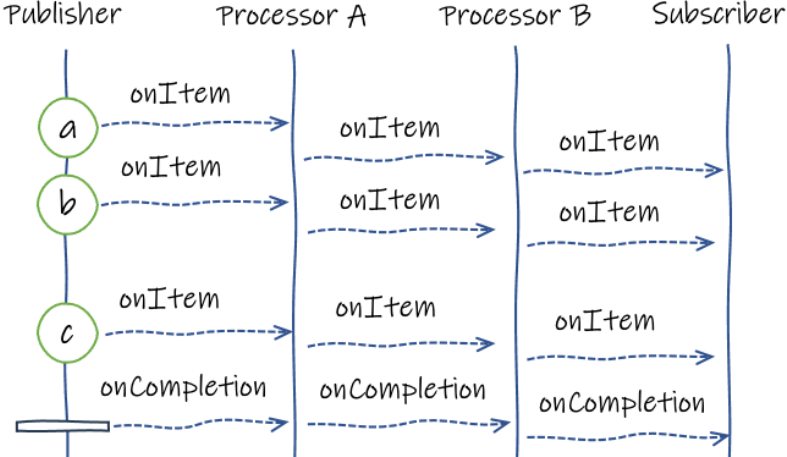
\includegraphics[width=0.9\textwidth]{EventFlow}
  \caption{Exemplarische Abbildung eines Event Flow in der Reactive Programming-Bibliothek Mutiny \parencite{MutinyEventFlow}}
  \label{fig:eventflow_mutiny}
\end{figure}

Nicht-blockierende, asynchrone Ein- und Ausgabe ist das Grundkonzept reaktiver Programmierung.

Dabei wird nach dem Start der Übertragung bereits begonnen die Teile des Programms auszuführen, die nicht von dem Ergebnis der I/O Operation abhängen.
Bei synchroner bzw. blockierender Ein- und Ausgabe hingegen wird die restliche Ausführung des Programms blockiert
bis die Datenübertragung abgeschlossen ist.

\begin{lstlisting}[caption=Pseudocode Nonblocking I/O (NIO), captionpos=b, label=lst:NIO_Pseudocode]
NonBlockingDatabaseRequest().subscribe(print("req finished"))
NonBlockingDatabaseRequest2().subscribe(print("req 2 finished"))
print("hello world")
\end{lstlisting}
In Listing \ref{lst:NIO_Pseudocode} kann durchaus zuerst \verb|hello world| ausgegeben werden da die gestarteten Datenbank-Anfragen die
restliche Programmausführung nicht blockieren. Wenn statt \verb|hello world| versucht werden würde die Ergebnisse einer der Datenbank-Abfragen
darzustellen, wäre das Ergebnis möglicherweise eine Exception oder \verb|null|, da die Anfragen zur Zeit der Ausführung von Zeile 3 noch nicht notwendigerweise
abgeschlossen wäre. Das ist ein gängiger Fehler beim Arbeiten mit asynchronen, nicht-blockierendem Programmcode.

\subsection{Vorteile und Nachteile}
\label{subsec:vorteile_nachteile}

Die Vorteile der Nutzung von einigen wenigen \verb|kernel threads| als \verb|IO Threads| gegenüber eines ganzen Threadpools
an \verb|kernel threads|, um einen \verb|kernel thread| an jede HTTP-Anfrage zu binden, liegen insbesondere in den Antwortszeiten bei
hoher Last und dem Ressourcenverbrauch.
Umso weniger \verb|kernel threads| gleichzeitig aktiv sind, desto weniger Threadwechsel auf Betriebssystemebene
gibt es auch pro CPU-Kern.

Da Threadwechsel nicht mehr der limitierende Faktor sind und jeder \verb|IO Thread| wesentlich mehr CPU-Rechenzeit nutzen kann,
skalieren die Antwortzeiten von Anwendungen wesentlcih besser mit der Erhöhung der Last.
Darüber hinaus sinkt auch der allokierte Speicher deutlich
\footnote{Eine 64 Bit-JVM reserviert auf Linux-und Solaris-Systemen standardmäßig 1 MB Speicher für den Threadstack eines Threads}
und der Grad der Parallellität wird nicht mehr von der Anzahl der verfügbaren Threads begrenzt.

Die Umstellung auf das reaktive Programmierparadigma erfordert allerdings eine Änderung in der Denk- und Herangehensweise bei der
Entwicklung von Softwarekomponenten. Denn reaktive Komponenten haben in der Regel keinen Zustand,
sondern reagieren lediglich auf interne Änderungen in den zugrundeliegenden Datenströmen.
Die bisherigen Programmabläufe müssten daher als reaktive Pipelines neu konstruiert werden.

Darüber hinaus ist reaktiver Code schwieriger zu debuggen und zu testen als imperativer Code, denn die Programmlogik die in den einzelnen Operatoren
der \verb|Pipes| einer \verb|Pipeline| aufgerufen wird, besteht in der Regel aus anynomen Funktionen und ist daher schwierig im Stack Trace einer
\verb|Pipeline| zurückzuverfolgen.
Während \verb|Event Flows| bei kleinen Pipelines noch zu überblicken sind, können komplexe Pipelines, die sich über die ganze Anwendung erstrecken,
schnell zu Wartbarkeits- und Verständnisproblemen führen.
Reaktive Programmierung ist zudem mit einer steilen Lernkurve verbunden. Dies liegt unter anderem an dem aktuellen Interesse an skalierenden
Anwendungen und der damit oftmals einhergehenden falschen Verwendung von Begriffen und der Überladung des Begriffs \verb|Reactive Programming|.
Aber auch die Funktionsweise von asynchronem Code (siehe Listing \ref{lst:NIO_Pseudocode}) kann zu schwer nachvollziehbaren und
reproduzierbaren Fehlern führen. Beispielsweise kann falsch strukturierter Code eine NullPointer-Exception auslösen, weil
er auf Daten eines Services zugreift die zum Zeitpunkt des Aufrufes bei hoher Latenz noch nicht vorhanden sind, bei niedriger Latenz
allerdings schon.

Außerdem gibt es zum aktuellen Stand kaum allgemeine, herstellerunabhängige Fachliteratur zu dem Thema.
Durch die Vielzahl an lange existierenden Reactive-Programming Bibliotheken
\footnote{Diese sind größtenteils bereits vor der Entwicklung des \textit{Reactive Streams}-Standards entstanden}
haben sich darüber hinaus viele verschiedene Nomenklaturen und Vorgehensweisen etabliert.

Ein weiteres Problem besteht bei der Integration in bestehende Enterprise Anwendungen. Bibliotheken und Konzepte die Themen wie
Security, Transaktionen oder Tracing behandeln, führen oft blockierenden, threadgebundenen Code aus.
Jede Schicht einer Anwendung muss reaktiv konzipiert sein, da die Verarbeitung einer Anfrage, die blockierenden Code aus einer der
Schichten aufruft, ansonsten den ausführenden IO-Thread blockieren kann, wodurch dieser keine weiteren Anfragen bearbeiten kann und somit die gesamte Anwendung blockiert.
\newline\newline
Die wesentlichen Vor-und Nachteile lassen sich wie folgt zusammenfassen:
\newline
\newline
Vorteile
\begin{itemize}
  \item Die Antwortzeiten sind für hohe Lasten geringer, da deutlich weniger Threadwechsel gemacht werden müssen und jeder Thread
        mehr Rechenzeit bekommt
  \item Der Speicherverbrauch ist geringer, da weniger Threads genutzt werden
  \item Der Grad der Parallellität ist nicht von der Anzahl der Threads begrenzt
\end{itemize}
Nachteile
\begin{itemize}
  \item Asynchroner Code ist schwieriger zu schreiben, lesen, testen und zu debuggen als imperativer Code
  \item Sehr aufwendig in bestehende klassische Enterprise-Anwendungen zu integrieren
  \item Reaktive Anwendungen müssen in jeder Schicht reaktiv sein (Transaktionen, Security, Datenbanktreiber)
  \item Blockierende I/O-Operationen führen zur Blockierung des IO-Threads und damit zur Blockierung der gesamten Anwendung
\end{itemize}

\subsection{Reaktive Datenströme}
\label{section:reaktive_datenströme}
In einer typischen asynchronen Verarbeitungskette von potenziell unbegrenzten Datenströmen
,bestehend aus einem Sender und Empfänger bzw. Publisher und Subscriber, kann es vorkommen,
dass der Sender Daten schneller an den Empfänger verschickt, als dieser sie verarbeiten kann.
Zwei \verb|naive| Ansätze mit einer Überlastung des Empfängers umzugehen wären:
\begin{enumerate}
  \item Nur der Empfänger reagiert auf eine Überlast. Diese kann sich in einem Speicherüberlauf äußern oder, falls der Puffer des Empfängers eine Größenbeschränkung
        hat, im Verlust der empfangenen Daten
  \item Der Sender begrenzt im Voraus die Datenmenge die er an den Empfänger schickt. Da der Sender allerdings in der Regel nicht weiß wieviel der Empfänger
        verarbeiten kann, sendet er entweder zuviel (es entsteht eine Überlast) oder er sendet zuwenig, wodurch der Durchsatz geringer ist als nötig \parencite{JavaSpektrum2015}
\end{enumerate}
Die Lösung für dieses Problem wird \textit{Backpressure} genannt.
Dabei fordert der Empfänger die Daten entsprechend seiner Kapazitäten vom Sender an, wodurch dieser weiß wieviele Daten er maximal versenden darf.
Diese Mitteilung muss asynchron geschehen, da bei einer synchronen Kommunikation der Backpressure die Vorteile der asynchronen, reaktiven Datenverarbeitung
negiert wird.
Da große Anwendungen aus mehreren Schichten (bspw. Routing-Schicht, Persistenzschicht, Geschäftslogik) bestehen und somit zwischen
dem Sender und Empfänger mehrere Komponenten liegen können, muss jedes
Element der Verarbeitungskette nichtblockierendes, asynchrones Verhalten implementieren, da ansonsten der Rest der Kette blockiert wird.

Aus der Intention einen Standard für die asynchrone Verarbeitung von Datenströmen mit nicht-blockierender \textit{back pressure}
zu schaffen, ging die \textit{Reactive Streams}-Initiative hervor.
Innerhalb dieser Initiative haben sich mehrere Arbeitsgruppen gebildet, welche die grundlegenden Semantiken erarbeitet haben und
sie in Form einer eigenen Spezifikation namens \textit{Reactive Streams} für die JVM veröffentlicht haben.\parencite{ReactiveStreams}
Diese API wurde anschließend in Java 9 als Schnittstelle namens \textit{Flow-API} dem JDK hinzugefügt.
Die \textit{Flow-API} entspricht der \textit{Reactive Streams} Spezifikation und stellt (nur) Interfaces zur Verfügung mit denen eine
asynchrone, nicht blockierende Verarbeitung von (unbegrenzten) Datenströmen mit \textit{back pressure} auf der JVM implementiert werden kann.
\parencite{OracleFlow}.
\footnote{Nicht zu Verwechseln mit den Java-Streams durch die Collection-API ab Java 8. Diese sind zur Auswertungszeit in ihrer Größe begrenzt und
  nach der Abarbeitung liegt statt eines Streams eine Collection vor}

\subsubsection{Java Flow-API}
\label{subsection:java_flow_api}
Die Flow-API fügt die nicht instanziierbare Klasse \verb|java.util.concurrent.Flow| zur Standardbibliothek hinzu. Sie enthält 4 Interfaces um das beschriebene,
vom \textit{Reactive Streams}-Projekt standardisierte, Publisher-Subscriber Model des Daten- bzw. Eventflusses
(siehe Listing \ref{lst:eventflow_pseudocode} und Abbildung \ref{fig:eventflow_mutiny}) mit \verb|backpressure|
von reaktiven Anwendungen auszudrücken:
\begin{enumerate}
  \item Publisher
  \item Subscriber
  \item Subscription
  \item Processor
\end{enumerate}

Die \verb|Flow|-Klasse erlaubt es Komponenten zu implementieren, die Teil von reaktiven Pipelines sein können, in denen
\verb|Publisher| Elemente produzieren, die von einem oder mehreren \verb|Subscribern| konsumiert werden.
Die Beziehung zwischen einem \verb|Publisher| und \verb|Subscriber| wird durch eine \verb|Subscription| abgebildet.
Während ein \verb|Publisher| theoretisch eine unbegrenzte Menge an Events liefern kann, wird er durch den \verb|Backpressure|-Mechanismus eingeschränkt.
Dadurch liefert der \verb|Publisher| immer nur soviele Elemente wie vom \verb|Subscriber| gefordert.
Der \verb|Publisher| erlaubt einem \verb|Subscriber| sich bei ihm zu registrieren um über die herausgegebenen Events informiert zu werden.
Die Kontrolle über den Fluss an Elementen (flow control), inklusive \verb|backpressure|, zwischen einem \verb|Publisher| und einem \verb|Subscriber|
wird von einer \verb|Subscription| verwaltet.
In Listing \ref{lst:java_flowapi} werden die 4 Interfaces der Flow-API dargestellt:
\begin{lstlisting}[language=java, caption=Die Klasse java.util.concurrent.Flow, captionpos=b, label=lst:java_flowapi]
@FunctionalInterface
public static interface Flow.Publisher<T> {
	public void subscribe( Flow.Subscriber<? super T> subscriber );
}
public static interface Flow.Subscriber<T> {
	public void onSubscribe( Flow.Subscription subscription );
	public void onNext( T item );
	public void onError( Throwable throwable );
	public void onComplete();
}
public static interface Flow.Subscription {
	public void request( long n );
	public void cancel();
}
public static interface Flow.Processor<T,R>
extends Flow.Subscriber<T>, Flow.Publisher<R> {
}
\end{lstlisting}\parencite[Kapitel 5.11]{JavaSE9StandardBibliothek}

Die vier \gls{callback}(*)-Methoden des \verb|Subscriber|-Interface werden vom \verb|Publisher| aufgerufen sobald eines der jeweiligen Events ausgelöst wird.
Die Events müssen dabei immer in der gleichen Reihenfolge veröffentlicht, und die jeweiligen Callback-Methoden ausgeführt, werden:
\begin{enumerate}
  \item onSubscribe
  \item onNext*
  \item (onError | onComplete)?
\end{enumerate}
Die Notation bedeutet, dass \verb|onSubscribe| immer als erstes aufgerufen werden muss, gefolgt von einer beliebigen Anzahl an
\verb|onNext|-Aufrufen. Dieser Eventstrom kann theoretisch ewig weitergehen oder durch ein \verb|onComplete|-Aufruf, welcher
signalisiert das keine weiteren Elemente mehr vom \verb|Publisher| produziert werden, beendet werden.
Im Fehlerfall wird vom \verb|Publisher| das \verb|onError|-Callback aufgerufen.

Sobald sich ein \verb|Subscriber| bei einem \verb|Publisher| registriert wird zuerst die \verb|onSubscribe|-Methode aufgerufen und dann ein
\verb|Subscription|-Objekt zurückgegeben. Ein \verb|Subscription|-Objekt wird nur von genau einem \verb|Subscriber| und einem \verb|Publisher| genutzt
und bildet die einzigartige Beziehung zwischen ihnen ab.

Der \verb|Subscriber| kann die \verb|request|-Methode des \verb|Subscription|-Interfaces nutzen um den \verb|Publisher| zu informieren das er bereit
ist eine gegebene Anzahl an Events zu verarbeiten (backpressure). Mit der \verb|cancel|-Methode kann er die \verb|Subscription| abbrechen und dem \verb|Publisher|
somit mitteilen das er nicht länger Events erhalten will.
\parencite{OracleFlow}

Das \verb|Processor|-Interface erweitert \verb|Publisher| und \verb|Subscriber| ohne das weitere Methoden implementiert werden müssen.
Dieses Interface repräsentiert eine Transformation der Events die durch den
reaktiven Datenstrom verarbeitet werden (siehe Listing \ref{lst:eventflow_pseudocode}).
Klassen die dieses Interface implementieren repräsentieren in der Regel die Operatoren einer Reactive Programming-Bibliothek.
Sobald ein \verb|Processor| ein Fehler erhält kann er sich entweder davon erholen oder direkt das \verb|onError|-Signal an seinen
Downstream-Subscriber propagieren. Ein typischer Lebenszyklus eines reaktiven Datenstroms mit der Flow-API wird in
Abbildung \ref{fig:flow-api} gezeigt.
\begin{figure}[ht!]
  \centering
  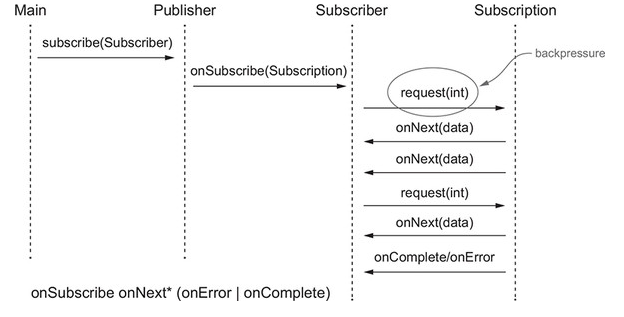
\includegraphics[width=0.9\textwidth]{flow-api_manning.PNG}
  \caption{Lebenszyklus eines reactive streams mit der Flow-API \parencite[Kapitel 17,  Figure 17.3]{JavaInAction}}
  \label{fig:flow-api}
\end{figure}
\newpage

\subsection{Reaktive Systeme}
\label{subsection:reaktive_systeme}
Anforderungen an große Softwaresysteme haben sich in den letzten Jahren stark verändert:
\begin{itemize}
  \item Antwortzeiten in Millisekunden statt im Sekundenbereich
  \item Datengrößen in Petabytes statt Gigabytes
  \item 100\% Verfügbarkeit statt stundenlange Wartungsarbeiten
  \item Deployment auf einer Vielzahl von Plattformen und cloud-basierten Clustern mit tausenden Multikernprozessoren
\end{itemize}

Unternehmen aus verschiedenen Bereichen haben sich voneinander unabhängig an diese Kriterien angepasst und Architekturmuster
erarbeitet, mit denen robuste, belastbare und flexible Softwaresysteme entwickelt werden können, welche diese modernen Anforderungen
erfüllen.

2014 wurde mit dem \verb|Reactive Manifesto| versucht, diese Ansätze der Systemarchitektur in Form eines Manifests zusammenzuführen
und daraus allgemeingültige Systemattribute abzuleiten.

\subsubsection{Eigenschaften}
\label{subsubsec:reaktive_systeme_eigenschaften}
Laut des \verb|Reactive Manifesto| sind Systeme reaktiv wenn sie folgende Eigenschaften besitzen:
\begin{itemize}
  \item Reaktionsschnell
  \item Widerstandsfähig (gegen Fehler)
  \item Elastisch
  \item Nachrichtengesteuert
\end{itemize}
Solche Systeme sind, laut den Autoren, flexibler, stärker entkoppelt und besser skalierbar als herkömmliche, nicht-reaktive Systeme.
Dies mache sie leichter zu entwickeln, zugänglicher für Veränderungen und deutlich fehlertoleranter.
\newline\newline
Die Autoren definieren die genannten Systemeigenschaften wie folgt:
\paragraph{Antwortbereit}Das System reagiert, falls überhaupt möglich, zeitgerecht. Antwortbereitschaft ist dabei die Grundlage für Funktion und
Benutzbarkeit. Es ermöglicht das schnelle Erkennen und Behandeln von Fehlern, indem verlässliche, zeitliche Obergrenzen für die Antworten von
Komponenten innerhalb des Systems geschaffen werden. Sobald eine Komponente nicht innerhalb des Zeitfensters antwortet, wird dies als Fehler gewertet und kann
entsprechend behandelt werden.
Der Fokus von reaktionsschnellen Systemen liegt auf konsistenten und schnellen Antwortszeiten. Darüber hinaus schaffen sie
verlässliche Obergrenzen um eine konsistente Qualität zu erreichen.
Dieses Verhalten vereinfacht Fehlerbehandlung, und erhöht das Vertrauen der Benutzer bezüglich der Interaktion.

\paragraph{Widerstandsfähig/Fehlertolerant}Das System bleibt auch bei Fehlern reaktionsschnell. Das gilt nicht nur für geschäftskritische, hochverfügbare Systeme -
jedes System das nicht fehlertolerant ist, wird nach Fehlern nicht mehr reaktionsfähig sein.
Widerstandsfähigkeit wird durch Replikation von Funktionalität bzw. Redundanz, Eingrenzung von Fehlern, Isolation von Komponenten und
Delegation von Verantwortung realisierbar.
Fehler werden innerhalb einer Komponente eingegrenzt und die Komponenten sind voneinander isoliert. Dadurch bleibt das Gesamtsystem stabil, selbst
wenn eine einzelne Komponente versagt.
Die Wiederherstellung jeder Komponente (self-healing) wird an eine andere, möglicherweise externe, Komponente delegiert.
Die Hochverfügbarkeit der Komponenten wird, wo notwendig, durch Redundanz gewährleistet.

\paragraph{Elastisch}Das System bleibt reaktionsschnell unter variierenden Arbeitslasten. Auf Änderungen der Arbeitslast wird durch
Anpassung der allokierten Ressourcen, insbesondere Replikation, reagiert. Das impliziert ein Systemdesign das keine zentralen Bottlenecks oder
Reibungspunkte hat, damit Komponenten problemlos repliziert und die Last darauf verteilt werden kann.
Reaktive Systeme unterstützen prädiktive, skalierende Algorithmen zur Ressourcenberechnung,
indem sie die Live-Messungen von leistungsrelevanten Systemmetriken als Eingabe nutzen.

\paragraph{Nachrichtenorientiert}Reaktive Systeme basieren auf dem asynchronen, nichtblockierendem Austausch von Nachrichten, um die Komponenten voneinander
abzugrenzen und dadurch eine lose Kopplung, Isolation und eine transparente Lokalisierung der Komponenten zu ermöglichen.
Aufgrund dieser Abgrenzung werden Fehler als Nachrichten an andere Komponenten delegiert.
Der Ansatz, jegliche Kommunikation der Komponenten durch das Übermitteln von Nachrichten zu implementieren, ermöglicht Elastizität,
indem er das Verteilen der Arbeitslast, die Kontrolle der Datenströme und, falls nötig, Anwenden von \textit{back pressure} erlaubt.
Die Kontrolle der Datenströme erfolgt durch das Überwachen der Nachrichtenwarteschlangen zur Laufzeit (\textit{message queues}).

Ortsunabhängigkeit bedeutet, dass Code und Semantik des Programms nicht davon abhängen, ob dessen Teile auf demselben Computer
oder verteilt über ein Netzwerk ausgeführt werden.
Reaktive nachrichtenorientierte Systeme erlauben eine effiziente Verwendung von Ressourcen, da Komponenten beim Ausbleiben von
Nachrichten vollständig inaktiv bleiben können, und sich nicht regelmäßig über neue Nachrichten informieren müssen.\parencite{ReactiveSystems}

Im Gegensatz zu Events haben Nachrichten immer ein klar definiertes Ziel.
Das bedeutet, dass sich ein ereignisgesteuertes System- oder eine Komponente auf adressierbare Event-Quellen konzentriert,
während ein nachrichtengesteuertes System auf adressierbaren Empfängern basiert.

In Abbildung \ref{fig:reactive-traits} wird das Zusammenspiel der Eigenschaften eines reaktiven Systems dargestellt.

\begin{figure}[ht!]
  \centering
  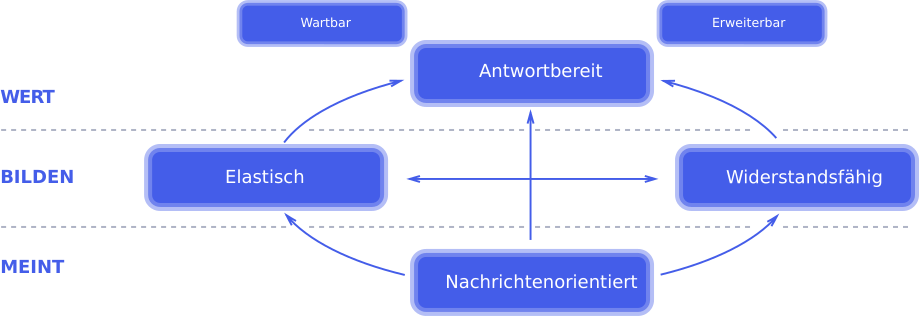
\includegraphics[width=0.9\textwidth]{reactive-traits-de}
  \caption{Zusammenspiel der Eigenschaften eines reaktiven Systems \parencite{ReactiveSystems}}
  \label{fig:reactive-traits}
\end{figure}
\newpage
\subsubsection{Abgrenzung zu reaktiver Programmierung}
\label{subsubsection:abgrenzung_reaktive_programmierung}
Aufgrund der steigenden Popularität von reaktiven Anwendungen ist der Begriff \verb|reaktiv| im Kontext der Softwareentwicklung
überladen und unterscheidet nicht zwischen \linebreak\verb|Reaktiver Programmierung| und \verb|Reaktiven Systemen|.

\verb|Reaktive Programmierung| ist eine ideale Technik zur Abbildung der internen Logik innerhalb einer Komponente in Form von Transformationen
auf Datenströmen, um sowohl Leistungsfähigigkeit, Ressourceneffizienz und Code-Verständlichkeit zu optimieren.

\verb|Reaktive Systeme| sind hingegen eine Menge von architektonischen Prinzipien, welche die verteilte Kommunikation hervorheben und
Ansätze zur Realisierung von Fehlertoleranz und Elastizität liefern.

Ein gängiges Problem bei ausschließlicher Nutzung von \verb|Reaktiver Programmierung| besteht darin, dass es die enge Kopplung
zwischen Verarbeitungsschritten (Transformationen) in einem eventgesteuerten Programm schwer macht, die geforderte Fehlertoleranz
eines reaktiven Systems zu erreichen.
Die Transformationsketten bzw. \verb|Pipelines| sind kurzlebig und die Operatoren und Callback-Methoden innerhalb der \verb|Pipes|
sind anonym, also nicht adressierbar.

Das bedeutet, dass sowohl Erfolg als auch Misserfolg bzw. Fehler direkt behandelt werden, ohne andere Komponenten darüber zu informieren.
Dieser Mangel an Adressierbarkeit erschwert die Wiederherstellung einzelner Phasen, da unklar ist, wo beziehungsweise ob Ausnahmen
propagiert werden sollten. Infolgedessen sind Fehler an kurzlebige Client-Anfragen und nicht an den
Gesamtzustand der Komponente gebunden – wenn eine der Phasen in der \verb|Pipeline| fehlschlägt, muss die gesamte \verb|Pipeline| neu
gestartet und der Client benachrichtigt werden. Dies steht im Gegensatz zu einem nachrichtengesteuerten reaktiven System, das
die Fähigkeit zur Wiederherstellung von Komponenten besitzt, ohne dass der Client benachrichtigt werden muss.

Ein weiterer Kontrast zum Ansatz eines reaktiven Systems ist, dass rein reaktive Programmierung zwar eine zeitliche Entkopplung,
aber keine räumliche Entkopplung ermöglicht. Zeitliche Entkopplung erlaubt gleichzeitige Verarbeitung, während räumliche Entkopplung
die Verteilung auf mehrere Systemkomponenten erlaubt. Dadurch können nicht nur statische, sondern auch dynamische Topologien
realisiert werden, was für die Elastizität eines reaktiven Systems essentiell ist.

Insgesamt ist \verb|reaktives Programmieren| eine sehr nützliche Technik, die in einer reaktiven Architektur genutzt werden kann.
Das Implementieren von Datenflüssen durch asynchrone und nichtblockierende Ausführung innerhalb eines Services kann die
die Basis eines reaktiven Systems bilden, mehrere reaktive Services bilden aber nicht direkt kein reaktives System.

Sobald mehrere Services in einem solchen System miteinander arbeiten sollen, müssen unter anderem Funktionalitäten wie
Datenkonsistenz, serviceübergreifende Kommunikation, Versionierung, Orchestrierung, Fehlermanagement und Trennung von Verantwortlichkeiten
berücksichtigt werden.

\subsection{Java Ökosystem}
\label{subsec:java_ökosystem}
Im Java Ökosystem gibt es eine Vielzahl an Libraries und Frameworks mit denen
\verb|Reaktive Programmierung| und \verb|Reaktive Systeme| umgesetzt werden können.
Um in Java einzelne, asynchrone Prozesse zu implementieren, wird vom JDK die Future-API zur Verfügung gestellt.\parencite{OracleFuture}
Für die Verarbeitung von asynchronen (unbegrenzten) Datenströmen gibt es die Interfaces der Flow-API (siehe Kapitel \ref{subsection:java_flow_api}).
\parencite{OracleFlow}

Im Folgenden wird ein Überblick über die Vielzahl an Bibliotheken und Frameworks gegeben.
\subsubsection{Reaktive Datenströme - Bibliotheken}
\label{subsubsec:reactive_streams}
Da die Flow-API lediglich Interfaces bereitstellt, gibt es mehrere Implementierungen von \verb|Reaktiven Datenströmen|.
Zu den populärsten Bibliotheken zählen:
\begin{itemize}
  \item RxJava
  \item Spring Webflux
  \item Mutiny
\end{itemize}
Jedes Projekt unterscheidet sich dabei in den verwendeten Klassen - und Operatoren, um die \verb|reactive streams|-Spezifikation,
beziehungsweise die \verb|Flow-API| des JDK, und damit auch \verb|back pressure| zu implementieren.
Trotzdem sind sie interoperabel und bieten in der Regel Converter-Klassen an.
\begin{itemize}
  \item RxJava\footnote{Implementiert die Flow-API erst seit Version 2} - Flowable, Observable \parencite{RxJava}
  \item Project Reactor - Flux, Mono \parencite{ProjectReactor}
  \item Mutiny - Multi, Uni \parencite{Mutiny}
\end{itemize}

\subsubsection{Reaktive Systeme - Toolkits}
\label{subsubsec:reaktive_systeme}
Für die Entwicklung von reaktiven Systemen bieten sich mehrere Toolkits an.
sie implementieren bereits Mechanismen wie Messaging, Event Loops,
nichtblockierende Netzwerkkomponenten und Dateizugriffe, sowie umfangreiche Funktionen für Webanwendungen.
Zu den populärsten gehören:
\begin{itemize}
  \item Eclipse Vert.x \parencite{Vert.x}
  \item Akka \parencite{Akka}
  \item Reactor-Netty \parencite{ProjectReactor}
\end{itemize}
Sowohl \verb|Eclipse Vert.x| als auch Reactor-Netty nutzen dabei \verb|Netty|
(siehe Kapitel \ref{subsubsec:reactor_pattern}) als Low-Level Framework für \verb|Nonblocking I/O|.
Da das in dieser Arbeit verwendete Anwendungsframework \verb|Quarkus| auf \verb|Eclipse Vert.x| basiert, wird Vert.x im Folgenden genauer beschrieben:

\paragraph{Eclipse Vert.x}
Vert.x ist ein Toolkit für das Entwickeln von reaktiven Anwendungen auf der JVM und wird durch die herstellerneutrale Eclipse Foundation entwickelt.
Da es sich nicht um ein Framework handelt, gibt es keine vordefinierte Grundlage für Anwendungen und dadurch kann es auch in bestehende Projekte
integriert werden.
Der Kern des Toolkits \verb|vertx-core| stellt APIs für asynchrones Programmieren, \verb|Nonblocking I/O|, Streaming und Zugriff zu
Netzwerkprokollen wie TCP, UDP, DNS, HTTP oder WebSockets zur Verfügung.
\begin{figure}[ht!]
  \centering
  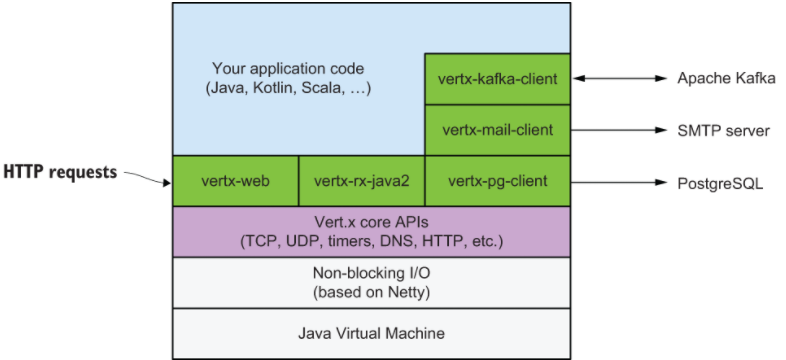
\includegraphics[width=1.0\textwidth]{vertx}
  \caption{Vert.x Struktur \parencite{Ponge2020}}
  \label{fig:vertx}
\end{figure}

Für die räumliche Entkopplung eines reaktiven Systems bietet Vert.x einen \verb|Event Bus|.
Der \verb|Event Bus| stellt ein verteiltes Peer-To-Peer Nachrichtensystem dar, welches sich über mehrere Serverknoten erstreckt.
Damit können verschiedene Komponenten eines Systems, unabhängig von der genutzten Programmiersprache, durch eindeutige Addressierung miteinander kommunizieren.
Auf jede Adresse können sich, ganz nach dem \verb|Publish-Subscribe|-Modell, mehrere Subscriber registrieren. Sobald Nachrichten an eine
Adresse veröffentlicht (published) werden, werden diese an jeden \verb|Subscriber| weitergeleitet.

Für die Resilienz eines reaktiven Systems verfügt Vert.x über einen Hochverfügbarkeits-Modus (high availablity, HA).
Dabei wird im Falle des Versagens einer Vert.x-Instanz die Anwendung auf eine andere Instanz innerhalb eines Clusters redeployed.
Darüber hinaus wird beim Ausfall einer Komponente durch einen \Gls{circuitBreaker}(*) vermieden, dass weitere Anfragen an diese
Komponente getätigt werden.\newline

Eine Implementierung des \verb|Reactor|-Pattern nutzt standardmäßig einen einzigen \newline\verb|Event loop thread|,
der in einer Schleife alle Events an die jeweils registrierten Event-Handler liefert.
Da durch einen einzigen \verb|Event loop thread| allerdings zu jeder Zeit auch nur ein CPU-Kern genutzt wird, kann
eine solche Implementierung Mehrkern-CPUs nur nutzen, indem mehrere Prozesse gestartet und verwaltet werden.

Statt einer einzigen Event Loop hält jede Vertx-Instanz, abhängig von der Anzahl der verfügbaren CPU-Kerne\footnote{1 Thread pro logischem CPU-Kern},
mehrere \verb|Event loop threads|. Diese Threads werden aus einem im vornherein erzeugten \verb|Event loop thread pool| entnommen.
\footnote{Die Größe des \textit{event loop thread pools} kann auch manuell überschrieben werden}

Um dieses Pattern vom Single Threaded Reactor-Pattern zu unterscheiden, wird es in der Vert.x-Dokumentation als \verb|Multi-Reactor Pattern| bezeichnet.
\parencite{Vert.xDocs}  \newline

Im Falle, dass die Event Loop eines \verb|Event loop threads| durch \verb|Blocking I/O| blockiert wird, wird die Operation stattdessen auf einem
\verb|Worker thread|, aus einen im vornherein erzeugten \verb|Worker thread pool|, abgewickelt. Diesen Prozess bezeichnet \verb|Vert.x| als \verb|Dispatching|.
Durch \verb|Dispatching| entstehen unvermeidbare Threadwechsel, aber es ermöglicht die Nutzung von Vert.x in bestehenden Projekten, die nicht komplett
auf \verb|Nonblocking I/O| basieren\parencite[Seite 2]{VertxArticle}.
Vert.x führt also zwei Thread Pools mit \verb|Kernel-Threads|, einen für \verb|Event loop threads|, dessen Größe der Anzahl der logischen CPUs entspricht,
und einen für \verb|Worker threads|, auf dem die Operationen abgearbeitet werden, welche die \verb|Event loop threads| blockieren würden.
\parencite{Vert.xOptions}

\subsubsection{Frameworks}
\label{subsubsec:frameworks}
Um komplette Web-Applikationen zu implementieren bietet sich der Gebrauch von Frameworks an, die Entwicklern viele grundlegende Architekturentscheidungen
abnehmen und bereits vorgefertigte Lösungen für Themen wie Authenfizierung, Routing, \Gls{ormg}(*), Security und Serialisierung anbieten oder
Lösungen von Drittanbietern integrieren und vorkonfigurieren.
Um reaktive Anwendungen und Systeme mit mehreren Services sinnvoll zu nutzen, ist es notwendig dass jede, für die Abarbeitung eines Requests relevante,
Anwendungsschicht und Komponente auch reaktiv ist und \verb|Nonblocking I/O| benutzt, sowie eine API bietet auf der
sich Event-Handler bzw. Subscriber registrieren können.\newline
Die populärsten Frameworks mit einem komplett reaktiven Stack sind dabei:

\begin{itemize}
  \item Spring WebFlux
  \item Quarkus
\end{itemize}

Spring WebFlux nutzt dabei \verb|Project Reactor| und Quarkus \verb|Vert.x| als reaktive Engine. \parencite{QuarkusReactiveGettingStarted}
Da die exemplarischen Anwendungen dieser Arbeit (siehe Kapitel \ref{section:vergleich_reaktiv_blockierend}) das Quarkus-Framework nutzen, wird dies
im Folgenden genauer beschrieben:
\paragraph{Quarkus und native image}

Bei dem, in dieser Arbeit verwendeten, Framework \verb|Quarkus| handelt es sich laut Hersteller \textit{Red Hat} um ein
benutzerfreundliches, auf Entwickler abgestimmtes Java Framework, welches für Container-, Cloud- und Serverless-Umgebungen optimiert ist und nur wenig
Konfiguration benötigt. Dabei werden nur die besten und hochwertigsten Java-Bibliotheken und Standards verwendet.
Dabei können die Anwendungen sowohl auf einer JVM (JVM mode) laufen, als auch, durch native Kompilierung mit vollständigem Stack,
als nativ ausführbare Anwendung: dem \textit{native image} (native mode).

Dafür nutzt Quarkus eine von Oracle entwickelte Technologie namens \verb|GraalVM|.
Dabei handelt es sich um eine polyglotte, virtuelle Maschine und Laufzeitumgebung die auf dem OpenJDK basiert, und über
JVMCI \footnote{Java Virtual Machine Compiler Interface} den C2-Compiler der zugrundeliegenden HotSpot-JVM durch den
polyglotten Graal Compiler ersetzt.\parencite{GraalVM}
Beim C2-Compiler handelt es sich um einen aggressiv optimierenden \verb|just-in-time|-Compiler (JIT) für Serveranwendungen, bei denen es nicht auf
schnelle Startzeiten und geringen Ressourcenverbrauch, sondern auf höchsten Durchsatz ankommt.
Dabei wird der unoptimierte Bytecode während der Laufzeit in Maschinencode übersetzt und ausgeführt. Sobald eine Methode hinreichend oft
ausgeführt wurde, daher auch als \verb|JIT Warm up| bezeichnet, und der Profiler genügend Informationen gesammelt hat, kann der JIT-Compiler
sie entsprechend optimieren bevor sie in Maschinencode übersetzt wird.
Der Graal Compiler kann sowohl als JIT-Compiler im JVM mode genutzt werden als auch als \verb|ahead-of-time|-Compiler (AOT) im native mode.\newline

Um ein \verb|native image| zu erstellen wird mithilfe des GraalVM-Compilers vor der Kompilierung der Anwendung in Maschinencode, also \verb|ahead-of-time|,
ermittelt, welche möglichen Pfade das Programm bei einem gegebenen Klassenpfad durchlaufen kann. Da dadurch nur die tatsächlich benötigten Klassen
kompiliert werden, sind Programme, die mit \verb|native image| erstellt wurden, um einige Größenordnungen kleiner als die Summe aus
JDK und den benötigten Bibliotheken.
Allerdings dauert der Vorgang aufgrund der umfassenden Analyse auch wesentlich länger als die Übersetzung in Bytecode mit \verb|javac|.
Damit Entwickler sich bei Java Anwendungen auch weiterhin nicht um Speicher-und Threadverwaltung kümmern müssen, wird die \verb|SubstrateVM|, eine
leichtgewichtige virtuelle Maschine, in das \verb|native image| hineinkompiliert.
sie stellt Laufzeitkomponenten wie den Garbage Collector und den Thread Scheduler bereit.

Die Analyse vor dem Kompilieren erfolgt unter der \verb|closed world|-Annahme. Dabei wird angenommen das jeglicher Code der zur Laufzeit des Programms
erreichbar ist zur Build-Time des \verb|native image| bekannt sein muss. Dadurch verursachen jegliche Java-Features die erst zur Laufzeit,
und nicht bereits während des Builds,
auswertbar sind, wie beispielsweise Reflection oder statische Initialisierung mit Datumswerten, Probleme für die Ahead-of-Time-Übersetzung.

Um dem Compiler die notwendigen Informationen zur Unterstützung von Reflection mitzuteilen, können
diese über Konfigurationsdateien oder programmatisch, über die GraalVM- und SubstrateVM-API hinterlegt werden.
Dadurch können auch Anwendungen und Libraries, wie beispielsweise Hibernate, Netty oder Tomcat,
die starken Gebrauch von Reflection machen so angepasst werden, dass sie in einem \verb|native image| genutzt werden können.
\parencite{GraalVMNativeImage}
Darüber hinaus verspricht Quarkus mit seiner Container-first-Philosophie durch \verb|native images|, bis zu 300 Mal schnellere Startzeiten
und nur ein Zehntel des Speicherbedarfs im Vergleich zu traditionellen Java-Frameworks wie Spring Boot.
Dadurch stellt ein \verb|native image| eine signifikante Reduzierung der benötigten Ressourcen und Kosten
im Cloud-Umfeld gegenüber einer Java-Anwendung auf der JVM dar.
\parencite{RedHatQuarkusInfografik}

Allerdings ist der maximal mögliche Durchsatz (noch) deutlich niedriger gegenüber Anwendungen im \verb|JVM-Mode|, da durch die AOT-Kompilierung
auf adaptive Laufzeitoptimierungen wie JIT-Compiling verzichtet wird.
Der Leiter des GraalVM-Projektes hat allerdings in einer Diskussion auf GitHub erwähnt, dass es durch Profile Guided Optimizations (PGO)
theoretisch durchaus möglich sei, einen gleichwertigen Durchsatz zu erreichen\parencite{GraalWuerthinger}.

Bei PGO handelt es sich, wie bei JIT-Compiling auch, um Profiling-Daten die zur Laufzeit des Programms gesammelt werden.
Im Gegensatz zu einer JVM-Anwendung liegt ein native image jedoch als Maschinecode und nicht als Bytecode vor,
und kann daher zur Laufzeit nicht optimiert werden.

Aus diesem Grund wird zuerst ein erstes native image generiert und ausgeführt.
Die hierbei ermittelten Profiling-Daten werden anschließend der Generierung des zweiten native image als Parameter hinzugefügt,
wodurch die Optimierungen bereits während des Builds ausgeführt und in das executable hineinkompiliert werden können.\newline

Des Weiteren erlaubt Quarkus die Kombination von blockierendem und nicht blockierendem, reaktiven Code.
Dabei wird der Dispatching-Mechanismus von \verb|Vert.x| genutzt (siehe Kapitel \ref{subsubsec:reaktive_systeme}).
Sobald also eine \verb|Blocking I/O|-Operation aufgerufen wird, wird diese auf einem \verb|Worker thread| abgewickelt,
anstatt die \verb|Event Loop|, und damit den
gesamten \verb|Event loop thread| bzw. \verb|IO thread|, zu blockieren.
Für die reaktive Programmierung bietet Quarkus die bereits genannte Bibliothek \verb|Mutiny| an.\parencite{Quarkus}

\subsection{Alternativen}
\label{subsec:alternativen}
In Java 1.1 wurden Threads als sog. \verb|Green Threads| implementiert.
Dabei wurde die Möglichkeit, Threads vom Betriebssystem, also \verb|Kernel threads|,
verwalten zu lassen, gar nicht genutzt.
\verb|Green threads| waren stattdessen als \verb|user threads| implementiert,
dabei ist die Funktionalität
nicht im Kernel implementiert, sondern in einer Programmbibliothek im Userspace (siehe Kapitel \ref{subsubsec:user-threads}).
Da sich das Betriebssystem nicht um das Scheduling von user threads kümmert, wurde dies über einen eigenen
Scheduling-Algorithmus der JVM geregelt.\parencite{Oracle2010}
Ein \verb|Green Thread| existiert lediglich als Objekt innerhalb der JVM, und durch die virtuelle Speicherverwaltung entfallen
somit die aufwändigen, kostenintensiven Betriebssystemaufrufe beim
Erstellen eines Threads sowie bei Threadwechseln.
Die Threadwechsel der \verb|Green Threads| erfolgten ausschließlich innerhalb des Main-Threads, weswegen keine echte Parallelität
realisiert werden konnte, da immer nur ein Prozessorkern genutzt wurde.
Während der Vorteil dieses Modells darin lag, dass es keine 'echten' parallelen Zugriffe auf eine Resource innerhalb des JVM-Prozesses geben konnte
und die Synchronisation von Datenzugriffen daher leicht war, überwog schließlich der Umstand, dass keine Nutzung von mehreren Prozessorkernen
durch Multithreading möglich war. Deswegen wurden \verb|Green Threads| ab Java 1.3 zugunsten von Kernel-Threads entfernt.

Mit dem OpenJDK Projekt \verb|Project Loom| wurde die Idee, allerdings nun als Ergänzung zu Kernel-Threads,
wieder aufgegriffen.
Statt alle virtuellen Threads auf dem nativen Main-Thread auszuführen, werden diese von einer geringen Anzahl an
nativen \verb|worker threads|, die als Carrier\footnote{Ein Kernel-Thread der mehrere virtuelle Threads ausführt} eingesetzt werden, ausgeführt.
Deren Anzahl ist so gewählt, dass alle CPU Kerne durch Multithreading dauerhaft benutzt werden
können\footnote{In der Praxis laufen natürlich noch andere Prozesse auf dem Server, deren Threads auch ausgeführt werden müssen.},
aber so wenig Kontextwechsel wie möglich ausgeführt werden müssen.\parencite{Oracle2021}
\footnote{Im Idealfall würde auf jedem CPU Kern ein \textit{worker thread} laufen, ohne Threadwechsel}
Während ein nativer Thread in einer 64 Bit JVM auf Linux-Systemen standardmäßig 1 MB für den Threadstack reserviert
, und zusätzlich noch Metadaten abspeichert, ist ein virtueller Thread
lediglich ein Objekt im virtuellen Speicher der JVM, weswegen er sehr wenig Ressourcen benötigt.
Aus diesem Grund können, bei entsprechend allokierten Heap-Speicher der JVM, durchaus mehrere Millionen virtueller Threads erzeugt werden, wohingegen
die Erstellung von 10.000 nativen Threads entweder den allokierten Speicher oder die Threadgrenze
des Betriebssystems überschreitet.\newline

In Kapitel \ref{subsubsec:user-threads} wurde bereits die Problematik erwähnt, sobald ein Kernel-Thread blockiert und somit
das Scheduling der Laufzeitumgebung nicht ausführen kann, weil ein darüber liegender \verb|user thread| bzw. virtueller Thread
eine blockierende I/O-Operation ausführt.
Dies würde bei mehreren Kernel-Threads bzw. Carriern wieder zu Threadwechseln seitens des Kernel-Schedulers führen.
Die vorgeschlagene Lösung besteht in der Nutzung einer asynchronen, nicht-blockierenden API für I/O Operationen von der Laufzeitumgebung.
Dadurch erhält der Aufrufer, in diesem Fall der Carrier, unverzüglich nach dem Start einer blockierenden I/O-Operation
innerhalb eines virtuellen Threads die Kontrolle zurück und kann währenddessen einen neuen virtuellen Thread bearbeiten.\newline
\verb|Project Looms| Versprechen ist allerdings eine Lösung zu finden die ohne asynchrone APIs für I/O-Operationen auskommt.
Diese gerade bei großen Systemen schwierig zu warten und zu verstehen.\newline

Ein virtueller Thread gibt in Project Loom freiwillig die Kontrolle an den Carrier ab (kooperatives Multitasking), wenn er auf I/O wartet und
dementsprechend pausiert. Dadurch blockiert er den Carrier nicht, der als Worker den virtuellen Thread ausführt.
Der Carrier führt dann durch einen virtuellen Threadwechsel den nächsten virtuellen Thread aus.
Das Basiskonzept für die Implementierung von virtuellen Threads in Project Loom wird als \verb|Delimited Continuation| oder \verb|Coroutine| bezeichnet.\newline
Eine \verb|Delimited Continuation| ist eine Folge von Anweisungen, die unterbrochen und später vom Aufrufer fortgesetzt werden kann.
Beim Unterbrechen durch die \verb|yield|-Methode der Continuation wird der aktuelle Zustand des ausführenden Threads
(Stack, Registerinhalte und Programmzähler) in eine Funktion umgewandelt.
Diese Funktion wird innerhalb der Continuation gespeichert, und die Kontrolle wird zurück an den Aufrufer gegeben.
Der Aufrufer kann nun zu einem späteren Zeitpunkt die \verb|run|-Methode der Continuation aufrufen.
Diese ruft die gespeicherte Funktion auf, und kann somit die Ausführung an der Stelle weiterführen, an der sie unterbrochen wurde.

Damit bieten \verb|Continuations| genau die Funktionalität, die für die Implementierung von virtuellen Threads in \verb|Project Loom| benötigt wird:
Ein Programm zu einem beliebigen Zeitpunkt anzuhalten, und später von diesem Punkt aus fortzusetzen.

Eine \verb|Continuation| ist also ein sehr mächtiges Konstrukt um den Programmfluss beliebig zu beeinflussen.

Um eine hohe Abwärtskompatibilität sowie möglichst geringen Migrationsaufwand für Entwickler zu gewährleisten, werden die Änderungen von
Project Loom in einer eigenen JDK Version bereitgestellt.
In dieser Version wurden viele Teile der Standardbibliothek die mit I/O-Operationen arbeiten, so angepasst, dass virtuelle Threads statt Kernel-Threads
genutzt werden. Auf diese Weise können I/O-Operationen, wie der Aufruf einer Netzwerkfunktionalität, die virtuellen Threads ohne Änderungen am Programm nutzen
und blockieren den darunterliegenden nativen Thread nicht mehr.
Im Folgenden werden die betroffenen Klassen genannt:\parencite{Oracle2021-Loom}

\begin{itemize}
  \item java.net.Socket
  \item java.net.ServerSocket
  \item java.net.DatagramSocket/MulticastSocket
  \item java.nio.channels.SocketChannel
  \item java.nio.channels.ServerSocketChannel
  \item java.nio.channels.DatagramChannel
  \item java.nio.channels.Pipe.SourceChannel
  \item java.nio.channels.Pipe.SinkChannel
  \item java.net.InetAddress
\end{itemize}